\documentclass[14pt,table]{extbook}
\usepackage[
%	showframe,
	a4paper, portrait, inner=3cm, outer=2cm, top=2.5cm, bottom=2.5cm]{geometry}

\setlength{\headheight}{17.0pt}

\usepackage{subfiles}
\usepackage{tikz}
\usepackage{lipsum}
\usepackage{float}
\usepackage{graphics}
\usepackage{pdfpages}
\usepackage{fancyhdr}
\usepackage{graphicx}
\usepackage{multicol}
\usepackage{multirow}
\usepackage{tabularx}
\usepackage{makecell}
\usepackage{microtype}
\usepackage{cellspace}
\usepackage{xcolor}
\usepackage[font={small,it}]{caption}
\usepackage[toc,page]{appendix}

\renewcommand\theadfont{\bfseries}

% Removes boxes from links
\usepackage[
    colorlinks=true,
    linkcolor=black,
    anchorcolor=black,
    citecolor=black,
    filecolor=black,
    menucolor=black,
    runcolor=black,
    urlcolor=black
]{hyperref}

% Disable default indentation an add paragraph spacing
\usepackage[parfill]{parskip}

\graphicspath{{images/} {../images}}

\input{definitions/000-plain-page-header-fix}
\input{definitions/001-center-page}
\usepackage{listings}
\usepackage{xcolor}

\definecolor{lst_frameborder}{rgb}{0.75, 0.75, 0.75}
\definecolor{lst_linenumbers}{rgb}{.5, .5, .5}
\definecolor{lst_codecomment}{rgb}{0, .8, .1}
\definecolor{lst_codekeyword}{rgb}{.5, .35, .05}
\definecolor{lst_codestrings}{rgb}{.8, 0, 0}
\definecolor{lst_codeidentif}{rgb}{0, .2, .6}

\lstset{
	basicstyle=\ttfamily\footnotesize,
	breaklines=true,
	numbers=left,
	numbersep=5pt,
	numberstyle=\ttfamily\footnotesize\color{lst_linenumbers},
	rulecolor=\color{lst_frameborder},
	tabsize=4,
	language=C,
	showspaces=false,
	showstringspaces=false,
	showtabs=false,
	frame=single,
	commentstyle    = \color{lst_codecomment},
	keywordstyle    = \color{lst_codekeyword},
	stringstyle     = \color{lst_codestrings},
	identifierstyle = \color{lst_codeidentif}
}
% Flowchart Shapes
% Original source from Overleaf
% https://www.overleaf.com/learn/latex/LaTeX_Graphics_using_TikZ%3A_A_Tutorial_for_Beginners_(Part_3)%E2%80%94Creating_Flowcharts

\usetikzlibrary{shapes.geometric, arrows}

\tikzstyle{startstop} = [rectangle, rounded corners, minimum width=3cm, minimum height=1cm, text centered, align=center, draw=black, fill=red!30]
\tikzstyle{io} = [trapezium, trapezium left angle=70, trapezium right angle=110, minimum width=3cm, minimum height=1cm, inner xsep=1pt, trapezium stretches=true, text centered, draw=black, fill=blue!30]
\tikzstyle{process} = [rectangle, minimum width=3cm, minimum height=1cm, text centered, align=center, draw=black, fill=orange!30]
\tikzstyle{decision} = [diamond, minimum width=3cm, minimum height=1cm, text centered, align=center, draw=black, fill=green!30]

\tikzstyle{state} = [ellipse, minimum width=3cm, minimum height=1cm, text centered, align=center, draw=black, fill=black!10]
\pgfkeys{/obi/fig/.is family, /obi/fig,
  default/.style = {caption=test}, % Initialize so 'defaults' exist
  caption/.store in = \figcaption,   % Any value assigned to foo will be stored in \foo
}

\newenvironment{obifig}[1]{\pgfkeys{/obi/fig/.cd, default, #1}\begin{figure}[H]\centering\vspace{1em}}{\caption{\figcaption}\end{figure}}
\pgfkeys{/obi/tab/.is family, /obi/tab,
  default/.style = {caption=test,size=\normalsize,cols=l},
  caption/.store in = \figcaption,
  cols/.store in = \obicols,
  size/.store in = \obitblsize
}

%% SNIPPET BEGIN
% Code courtesy of https://tex.stackexchange.com/a/14460/118294
\makeatletter
\newcolumntype{\expand}{}
\long\@namedef{NC@rewrite@\string\expand}{\expandafter\NC@find}
\makeatother
%% END SNIPPET

\newenvironment{obitab}[1]{
	\pgfkeys{/obi/tab/.cd, default, #1}
	\vspace{1em}
	\setlength{\tabcolsep}{0.5em}
	\begin{table}[H]
	\obitblsize
	\renewcommand{\arraystretch}{1.4}
	%\expandafter\tabular\expandafter{\obicols}
	\begin{tabular}{\expand\obicols}
}{
%	\endtabular
	\end{tabular}
	\caption{\figcaption}
	\renewcommand{\arraystretch}{1}
	\end{table}
}

\newcommand{\othead}[1]{
	
	\multicolumn{1}{c}{%\cellcolor{black}
	{
	\setlength{\tabcolsep}{0cm}
	\hspace{-1em}
	\setlength{\cellspacetoplimit}{0.7em}
	\setlength{\cellspacebottomlimit}{0.7em}	
	\begin{tabular}{@{}Sc@{}}
		\textcolor{white}{\textbf{#1}}
	\end{tabular}}}
}

\usepackage[cmintegrals,cmbraces]{newtxmath}
\usepackage{ebgaramond-maths}
\usepackage[T1]{fontenc}

\title{C: Zero To Hero - Programmer's Den Open Book Initiative}
\author{Tyler Dence, et. al.}
\date{April 2021}

\begin{document}

% Start book 
\frontmatter
    % Set page number to zero
    % This makes the cover take page zero,
    % which puts the first content at page 1.
    \setcounter{page}{0}
    
    % Set section depth to -1
    % Disables numbering on sections in the front matter
    \setcounter{secnumdepth}{-1}
    
    % Cover
    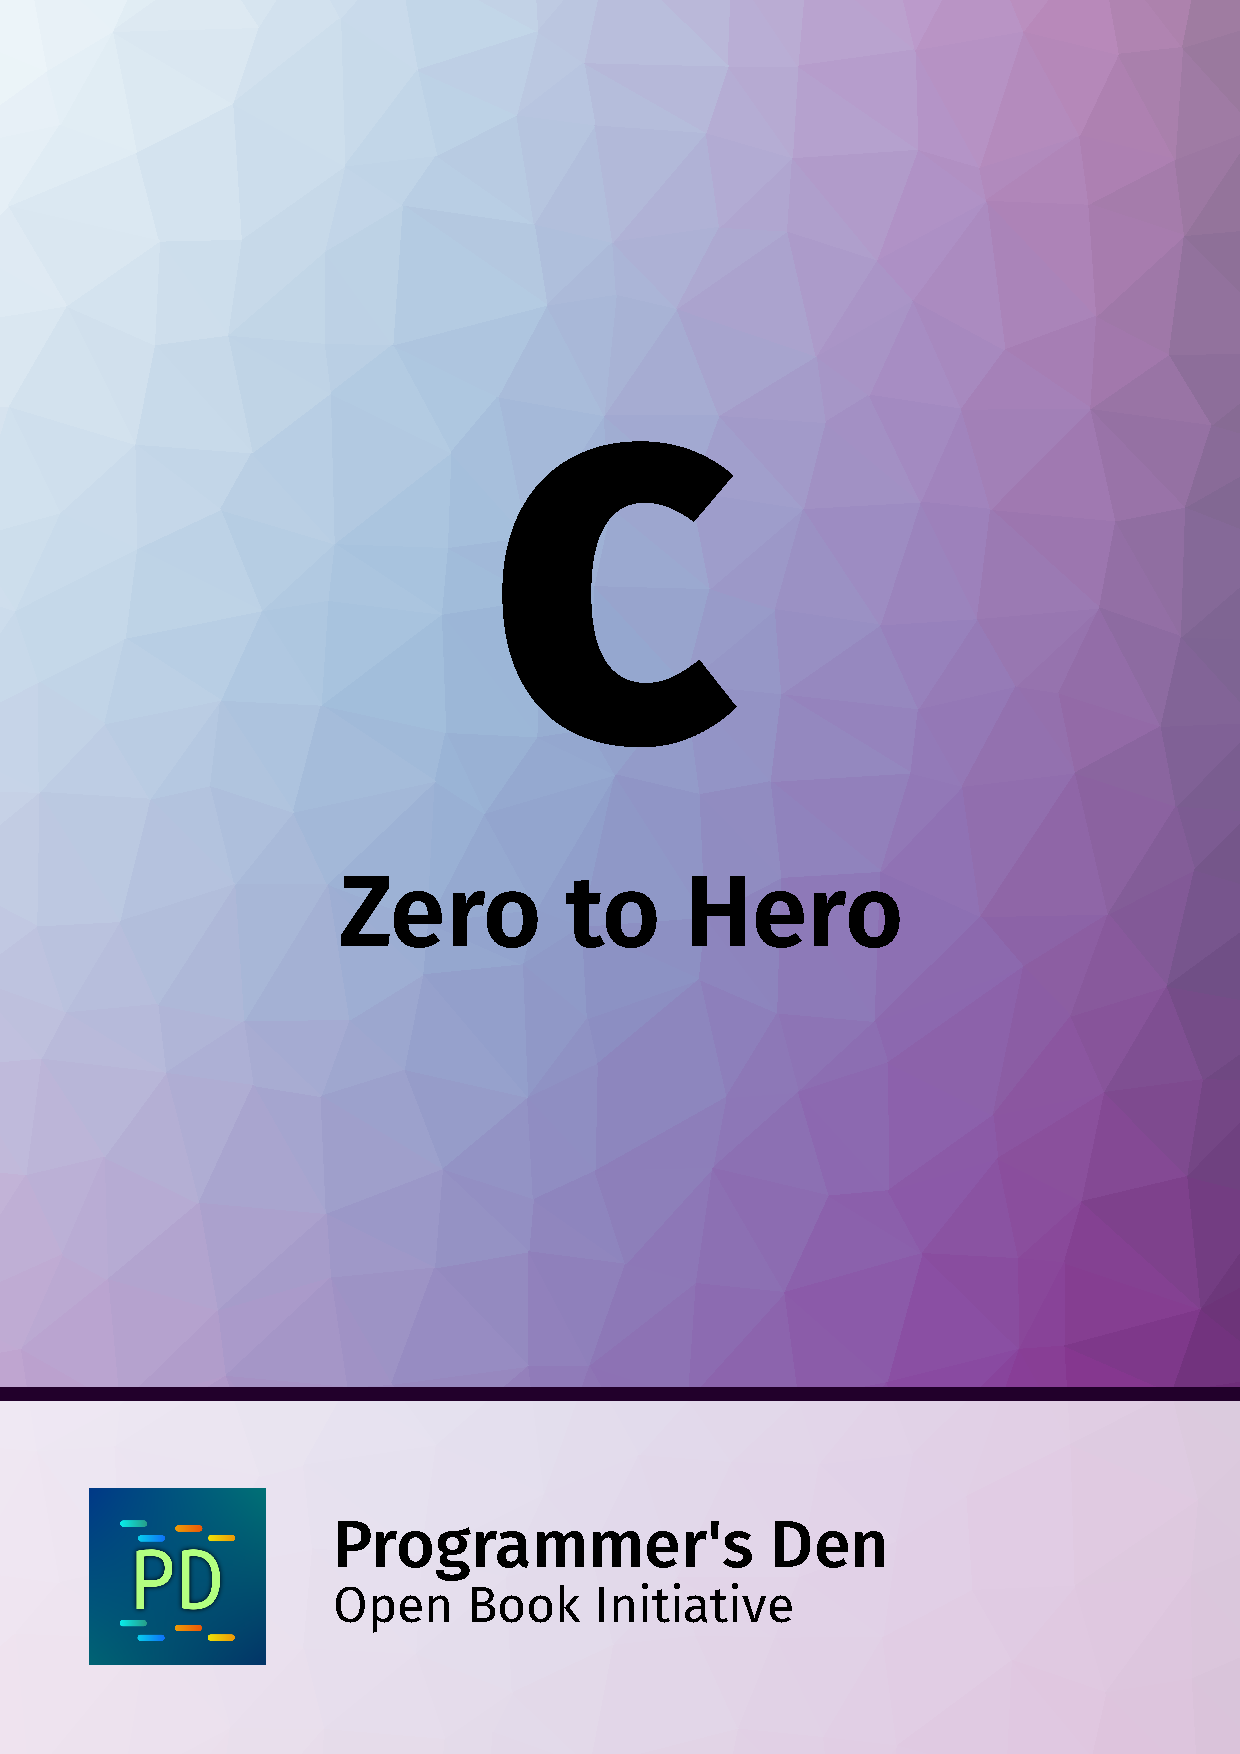
\includepdf[pages=-]{images/cover}
    
    % Front sections 
    \subfile{chapters/0.0-foreword}
    \subfile{chapters/0.1-copyright}
    
    % Create table of contents
    \tableofcontents
    
    % Fix header bug where "CONTENTS"
    % shows up in header of blank page
    % Note: bug only occurs if TOC takes
    % an odd number of pages to render
    \clearpage
    \markboth{}{}


    % Set section depth to 3
    % Re-enables section numbering
    \setcounter{secnumdepth}{3}

% Chapters
\mainmatter
	\part{The Basics}
		\subfile{chapters/1.0-introduction}
		\subfile{chapters/2.0-getting-started}

		\chapter{Control Structures}
			\section{Conditional Statements}
			\section{Loops}
				\subsection{While}
				\subsection{For}
				\subsection{Do-While}

		\chapter{Functions}
			\section{Method Signature}
			\section{Return Values}

		\chapter{Operators}
			\section{Arithmetic Operators}
			\section{Bitwise Operators}
			\section{Logical Operators}
			\section{Pointer Operators}
			\section{Operator Precedence (Order of Operations)}

		\chapter{C Type System}
			\section{Numerical Types}
				\subsection{Integers}
				\subsection{Floats}

			\section{Fixed-Width Data Types}

			\section{Textual Types}
				\subsection{Char}
				\subsection{Strings}

			\section{Custom Types}
				\subsection{Structs}
				\subsection{Unions}

		\chapter{Pointers}
			\section{Data Pointers}
			\section{Function Pointers}

	    \chapter{Memory Management}
	        \section{The Stack}
	        \section{The Heap}

	    \chapter{Data Structures}
	        \section{Arrays}
	        \section{Linked Lists}
	        \section{Vectors}

		\chapter{File I/O}
			\section{Reading Files}
			\section{Writing Files}

% Appendices
\appendix
	\subfile{chapters/A.0-setting-up}
	\subfile{chapters/B.0-dont-try-this-at-home}
	
	\chapter{Quick References}
		\section{Operator Table}
		\section{Data Types and Sizes}
		\section{Useful Constants}

\end{document}
